\documentclass{article}

\usepackage{graphicx}
\usepackage{amssymb, amsmath, amsthm}
\usepackage{physics}
\usepackage[shortlabels]{enumitem}
\usepackage{subcaption}

\author{Elnur Gasanov : 163411}
\title{HW 6 : Neural Networks}

\begin{document}
\maketitle

\section{Property of derivatives of error function}

\subsection{Sigmoid activation function}

First, let us calculate 

\begin{align}
\pdv{y}{a} = -\left(\frac{1}{1 + \exp(-a)}\right)^2 \cdot - \exp (-a) = y (1 - y).
\end{align}

Then note, that

\begin{align*}
\pdv{E}{a} &= \pdv{-(t \ln y + (1-t) \ln (1-y))}{a} = - \left(\frac{t}{y} \pdv{y}{a} - \frac{1-t}{1-y} \pdv{y}{a}\right) \\&= - (t(1-y) -(1-t)y) = y-t.
\end{align*}

\subsection{Softmax activation function}

Again, let us notice first that

\begin{align*}
\pdv{y_i}{a_k} = \begin{cases}
	-\frac{\exp(a_i)}{(\sum \exp(a_j))^2} \cdot \exp(a_k) = -y_i y_k, i \neq k, \\
	\frac{\exp(a_k) (\sum \exp(a_j)) - \exp^2(a_k)  }{(\sum \exp(a_j))^2} = y_k (1 - y_k), i = k.
	\end{cases}
\end{align*}

Then, taking derivative of $E$ with respect to $a_k$ we get that

\begin{align*}
\pdv{E}{a_k}& = - \pdv{\sum_j t_j \ln y_j}{a_k} = - \left(\sum_j \frac{t_j}{y_j} \pdv{y_j}{a_k}\right) \\
& = - \left(\left(\sum_{j \neq k} - t_j y_k \right) + t_k (1 - y_k) \right)\\
& = \left( \sum_j t_j \right) y_k - t_k = y_k - t_k.
\end{align*}

\subsection{Updating weights}

Gradients of $E(w)$ are often used to minimize the error function. After feeding forward a neural network a backpropogation step is run: starting from the output layer till the first hidden layer, errors on each node are calculated. Let edge connecting $k$-th node on the previous layer with $j$-th node on the next one ($i$ denotes some enumeration of layers) have the weight $w^i_{kj}$, similarly we denote the error on node as $\delta_k^i$. Then errors of nodes in the $i-1$-th layers are known given errors of next layer:

\begin{align*}
\delta^{i-1}_k = h'(\cdot)\sum_j w^i_{kj} \delta^i_j.
\end{align*}

Here $h'(\cdot)$ means the derivative of activation function on the node.

\section{Vanishing gradient problem}

\subsection{Description}

Let us look at the derivative of sigmoid function:

\begin{align*}
	\sigma'(x) = \left(\frac{1}{1 + \exp (-x)}\right)'= \frac{\exp (-x)}{(1 + \exp (-x))^2} = \sigma(x) (1 - \sigma (x)). 
\end{align*}

First, the derivative never exceeds $0.25$, since $\sigma(x) \in [0, 1]$. Second, the larger~$|x|$ , the smaller the derivative. Since the gradient consists of terms which are multiplied by the derivative of activation function, the gradient itself may be small what makes optimization process slow.

\subsection{Solutions}

\begin{enumerate}
	\item Use other activation functions, for example, ReLU or tanh;
	\item Add residual blocks;
	\item Add batch normalization layers (prevents $|x|$ to have large values);
	\item Initialize weights with small numbers
\end{enumerate}

\section{Neural Network}

\subsection{Description}

\# of inputs: 56, \# of outputs: 1, \# of hidden nodes: 40. Initially, weights were set randomly from normal distribution with zero mean and $\frac{1}{\sqrt{n}}$ std, where $n$ is the number of nodes in the corresponding layer.

\subsection{Training} 

Learning rate is 0.2. As can be seen from the plot, error decreases during learning.

\begin{figure*}
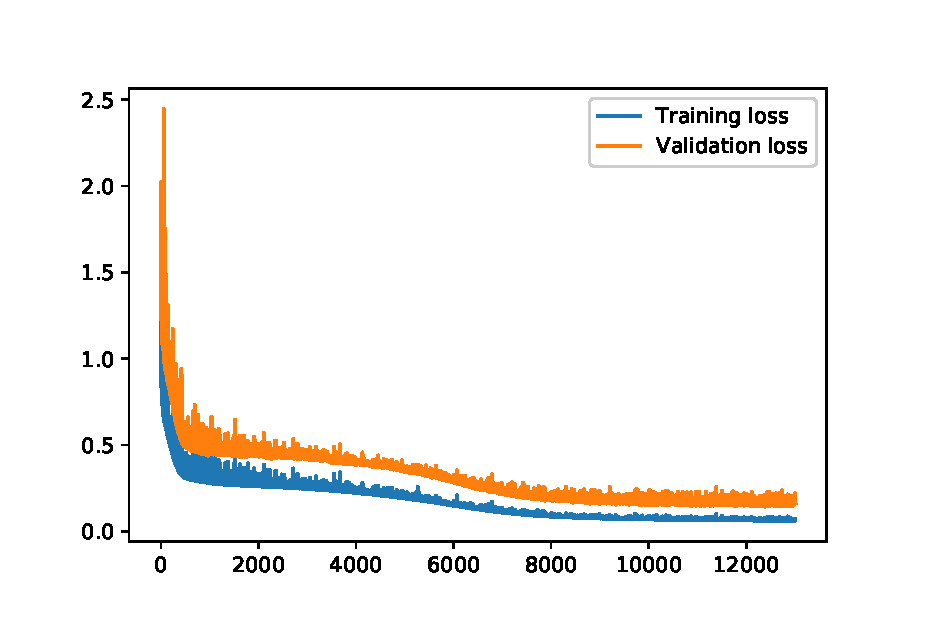
\includegraphics[width=\linewidth]{loss_decrease}
\caption{Train loss and validation loss s decreasing}
\end{figure*}

\subsection{Testing}

Mean error is 52.52, while standard deviation is 52.168. Plot shows how well test points are predicted. 

\begin{figure*}
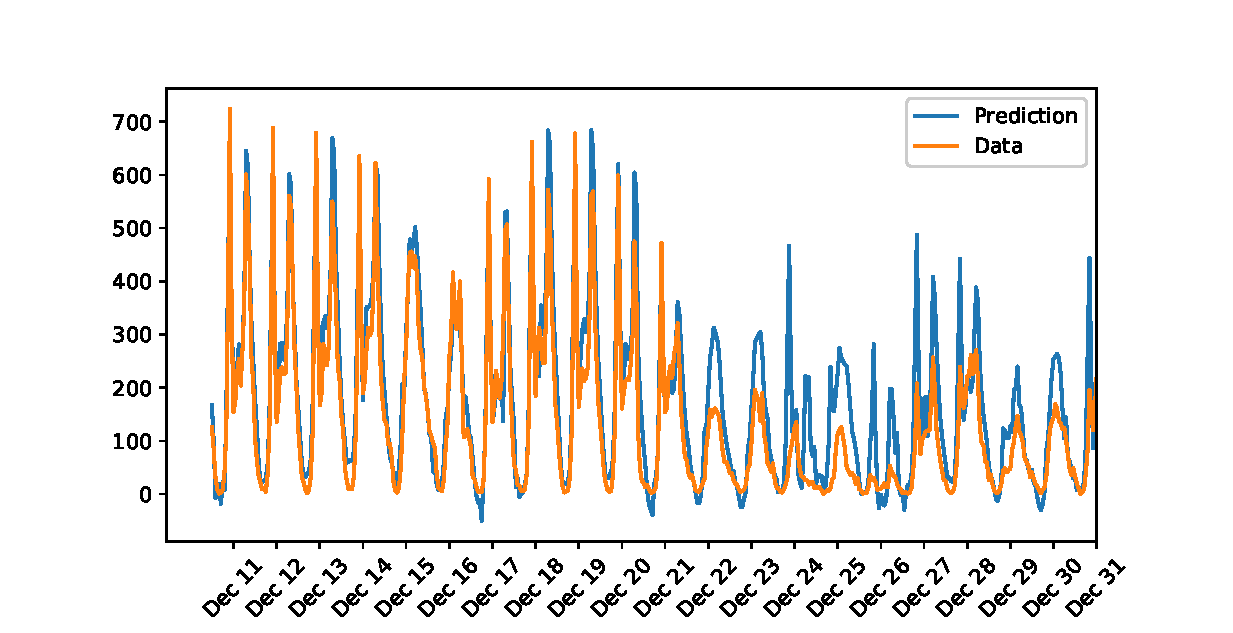
\includegraphics[width=\linewidth]{test}
\caption{Comparison of predictions and real labels on test data}
\end{figure*}

\subsection{Discussion}

It is important what we initialize weights in the beginning: if they are set to be numbers much further from zero, then we may have encountered vanishing gradient problem. Hidden nodes play a pivotal role here: if there are few of them, then NN may fail to derive all hidden features from the data, which may lead to an underfitting problem. But, on the other hand, the larger number of hidden nodes is, the heavier it is to train NN because of the length of a weight vector.

\section{Other optimization algorithms}

RMSProp and Adam algorithms were implemented. For RMSProp $\delta$s equal to 0.4 and 0.8 were tested. For Adam $\beta_1$ was set to 0.1, $\beta_2 = 0.2$. Loss decreases of both algorithms are shown in the figures below. Surprisingly, Adam optimizes loss function much faster than any algorithm which was used in this task. RMSProp does not show a good performance on the data.

\begin{figure*}
\centering
\begin{subfigure}{0.45\textwidth}
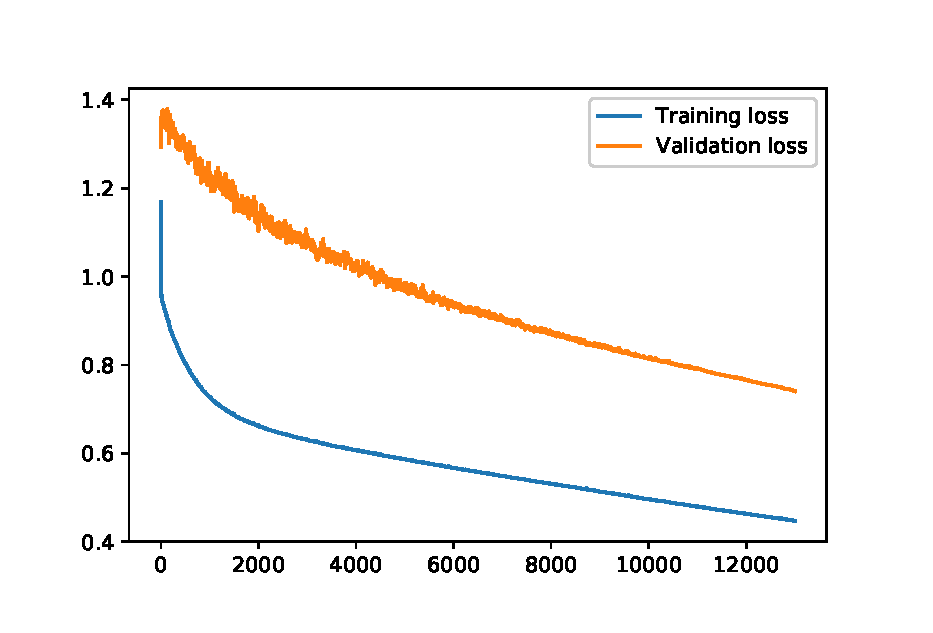
\includegraphics[width=\linewidth]{loss_decrease_rms_0.4.eps}	
\caption{$\delta=0.4$}
\end{subfigure}
~
\begin{subfigure}{0.45\textwidth}
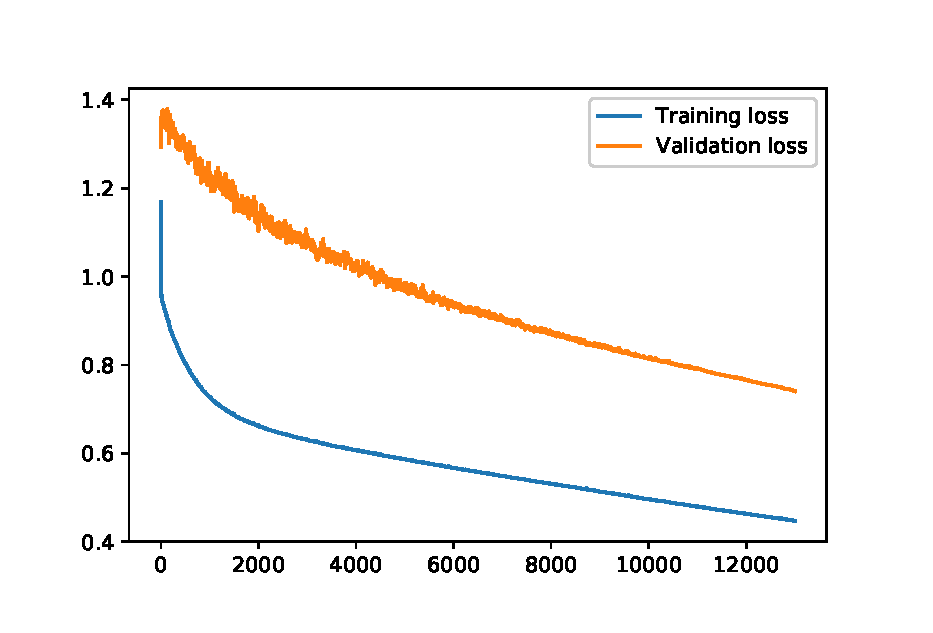
\includegraphics[width=\linewidth]{loss_decrease_rms_0.8.eps}	
\caption{$\delta=0.8$}
\end{subfigure}
\caption{RMSProp}
\end{figure*}

\begin{figure*}
	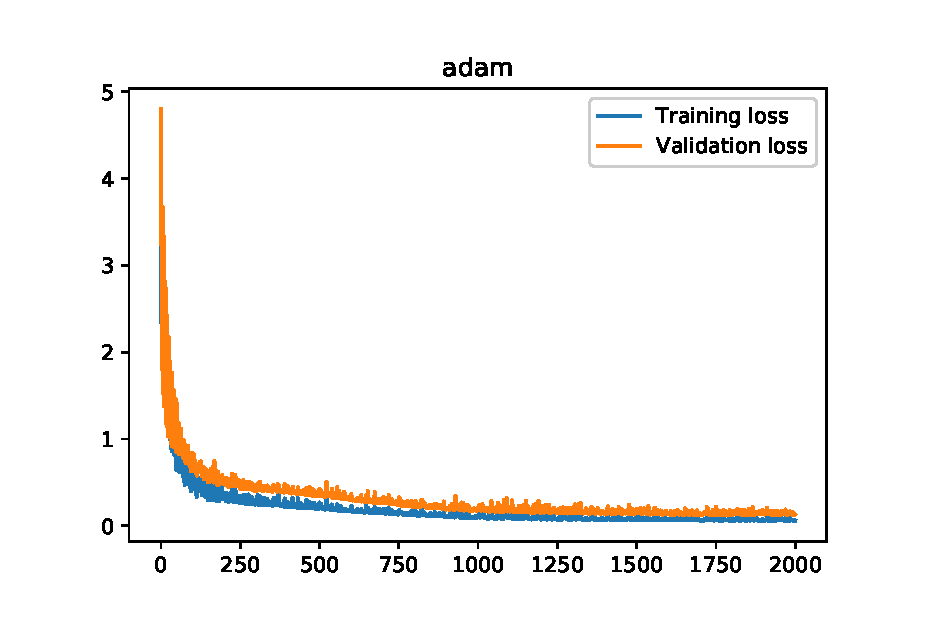
\includegraphics{loss_decrease_adam.eps}
	\caption{Adam needs only 2000 iterations to achieve a decent accuracy (training loss is less than 0.06)}
\end{figure*}



\end{document}